%% PolicyWatcher - SoftwareX Original Software Publication
%% Prepared from the official SoftwareX OSP LaTeX template (2026 version).
\documentclass[preprint,12pt,a4paper]{elsarticle}

\usepackage{amssymb}
\usepackage{booktabs}
\usepackage{graphicx}
\usepackage{hyperref}
\usepackage{tabularx}
\usepackage{xcolor}
\usepackage{array}

\hypersetup{hidelinks}

\setlength{\parindent}{0pt}
\setlength{\parskip}{4pt}
\setlength{\emergencystretch}{3em}
\urlstyle{same}
\newcommand{\pw}{\textsc{PolicyWatcher}}
\newcolumntype{Y}{>{\raggedright\arraybackslash}X}

\journal{SoftwareX}

\begin{document}

\begin{frontmatter}

\title{PolicyWatcher: Evidence-preserving monitoring of online terms and privacy policies}

\author[gsom]{Fabrizio Degni\corref{cor1}}
\ead{fabrizio.degni@gsom.polimi.it}
\ead[url]{https://www.policywatcher.online}
\cortext[cor1]{Corresponding author}
\address[gsom]{POLIMI Graduate School of Management, Via Lambruschini 4/c, Building 26/a, 20156 Milan, Italy}

\begin{abstract}
PolicyWatcher is open-source software for continuously retrieving, validating,
versioning, and communicating changes to online terms of service and privacy
policies. Its central design goal is to prevent plausible but unsupported data
from reaching public outputs. A five-path acquisition cascade combines direct
HTTP, explicit HTTP/2, optional browser rendering, and two timestamp-guarded web
archives. Retrieved pages pass content validation and provenance checks before
normalized text, hashes, diffs, and structured bilingual analyses are stored. A
shared public-evidence gate excludes development fixtures, partial retrievals,
and unverified records from pages, APIs, reports, search indexes, and subscriber
notifications. In a dated operational snapshot of 50 configured documents from
16 providers, 46 records passed the public-evidence gate and four were suspended;
a fixture-only control exposed no policy content or change records. The software
supports reproducible research on policy accessibility, retrieval-path
dependence, longitudinal change, and evidence-aware civic technology while
explicitly separating operational observations from claims about legal or
semantic accuracy.
\end{abstract}

\begin{keyword}
policy monitoring \sep web measurement \sep digital governance \sep provenance
\sep civic technology \sep research software
\end{keyword}

\end{frontmatter}

\section*{Required Metadata}

\section*{Current code version}

\begin{table}[!h]
\centering
\footnotesize
\setlength{\tabcolsep}{4pt}
\begin{tabularx}{\textwidth}{|p{0.055\textwidth}|p{0.285\textwidth}|Y|}
\hline
\textbf{Nr.} & \textbf{Code metadata description} & \textbf{Please fill in this column} \\
\hline
C1 & Current code version & v3.6.4, SoftwareX snapshot 1171b06 \\
\hline
C2 & Permanent GitHub link to code/repository used for this code version & \href{https://github.com/sev7enITA/policywatcher/tree/1171b06a119954343c9a9124df4bdfdc9aab4a6d}{GitHub commit 1171b06} \\
\hline
C3 & Legal Code License & MIT License \\
\hline
C4 & Code versioning system used & Git \\
\hline
C5 & Software code languages, tools, and services used & TypeScript, JavaScript, Next.js, React, Prisma, SQLite, Node.js, Playwright/Chromium, Google Gemini API \\
\hline
C6 & Compilation requirements, operating environments, and dependencies & Node.js 20 or later; npm; dependencies declared in \texttt{package-lock.json}; Chromium is needed only for the optional remote renderer \\
\hline
C7 & Link to developer documentation/manual & \href{https://github.com/sev7enITA/policywatcher/blob/1171b06a119954343c9a9124df4bdfdc9aab4a6d/README.md}{README at commit 1171b06} \\
\hline
C8 & Support email for questions & \href{mailto:fabrizio.degni@gsom.polimi.it}{fabrizio.degni@gsom.polimi.it} \\
\hline
\end{tabularx}
\caption{Code metadata (mandatory).}
\label{tab:metadata}
\end{table}

\section{Motivation and significance}
\label{sec:motivation}

Terms of service and privacy policies define how online services collect,
retain, transfer, and reuse information. Yet the documents are long, change over
time, and are rarely read in full. Prior work has quantified the reading burden
of privacy policies \cite{mcdonald2008}, documented user acceptance without
meaningful reading \cite{obar2020}, and created annotated or longitudinal
corpora for privacy research \cite{wilson2016,amos2021}. Systems such as Polisis
and CLAUDETTE analyze policy language \cite{harkous2018,lippi2019}, while
ToS;DR and TOSBack provide public summaries or tracked versions
\cite{tosdr,tosback}.

These contributions leave a practical research-software gap. Retrospective
corpora can fix their source set in advance, but a live monitor repeatedly faces
bot challenges, JavaScript-only pages, regional variants, URL changes, consent
interstitials, and archives that may be older than the current baseline. The
dominant failure is often not a crash. It is a plausible wrong document, such as
a challenge page or stale archive, that is stored and analyzed as if it were the
provider's policy.

\pw{} was developed to make that evidence boundary explicit. It monitors a
configured set of public legal documents and records how each observation was
obtained. It provides a running web application for citizens and practitioners,
but it is also research software: its retrieval logs, normalized versions,
provenance states, and public-evidence decisions can support studies of policy
accessibility, longitudinal change, and measurement reliability. The software
does not present model-generated explanations as legal advice, and its
operational measurements are not treated as a benchmark of legal interpretation
accuracy.

The user can deploy the application on commodity hosting, configure provider
URLs and jurisdictions, schedule bounded scans, inspect source-quality findings,
and publish only records that meet the evidence contract. Readers access a
bilingual public timeline, per-document diffs, comparison views, evidence-status
notices, and downloadable reports. Administrators additionally receive check
logs, dataset-quality findings, review history, and explicit controls for source
promotion or suspension.

\section{Software description}
\label{sec:description}

\subsection{Software architecture}

\pw{} is a server-rendered TypeScript application built with Next.js and React.
Prisma provides typed access to SQLite, while a small authenticated rendering
service can execute Chromium on infrastructure where a full browser runtime is
available. The hosted language model is an optional downstream analysis
component; acquisition, validation, hashing, evidence status, and public gating
do not depend on a successful model response.

Figure~\ref{fig:architecture} shows the evidence path. A scheduler submits each
configured URL to the acquisition cascade. The result is validated before any
text can enter the evidence store. Normalized text feeds hashing and diffing so
cosmetic markup changes do not become policy changes. Public outputs query a
shared gate rather than duplicating visibility logic at each page or API.

\begin{figure}[!ht]
\centering
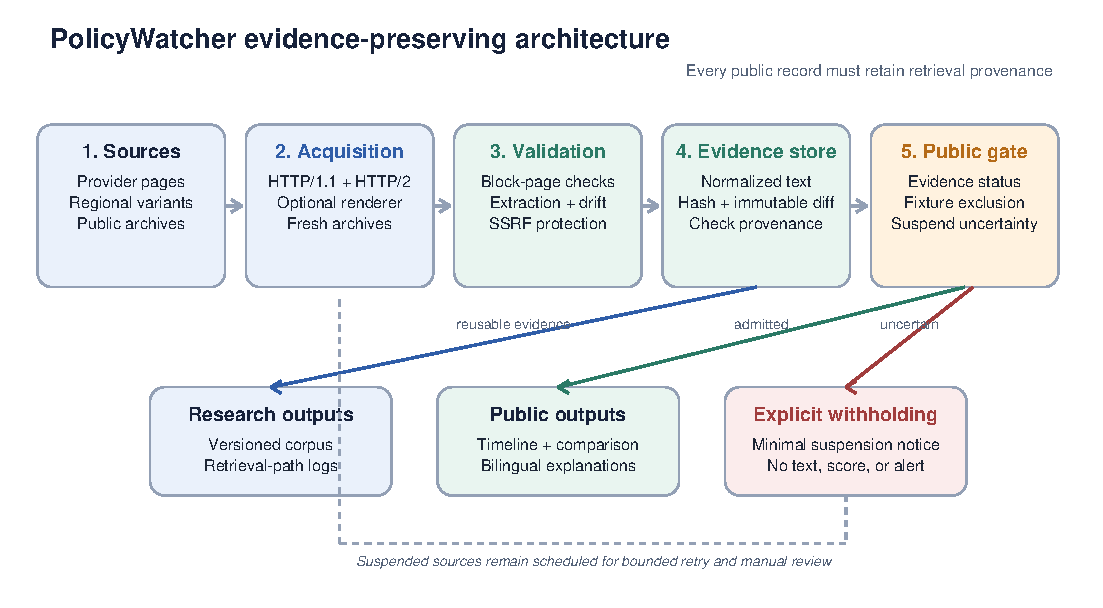
\includegraphics[width=\textwidth]{figures/architecture.pdf}
\caption{PolicyWatcher architecture. Retrieval provenance and evidence status
travel with each record; uncertain records follow the withholding path.}
\label{fig:architecture}
\end{figure}

\subsection{Acquisition and content contract}

The acquisition cascade orders five strategies by fidelity to the live source:
direct HTTP/1.1, explicit HTTP/2, optional headless rendering, the Wayback
Machine \cite{wayback}, and Common Crawl \cite{commoncrawl}. Direct requests use
bounded retries, body-aware timeouts, manual redirect handling, and address
validation at every hop. HTTP/2 is a separate path for servers that reject
non-browser HTTP/1.1 clients. The renderer executes script-dependent pages but
remains optional. Archives are witnesses of last resort.

Archive fallback is governed by a freshness rule: a candidate capture is
admissible only when its archive timestamp is not earlier than the last live
baseline. A stale capture therefore cannot replace a newer live document and
create a false regression. Captures without a usable timestamp are rejected.

Every retrieval returns exactly one of three states: \texttt{ok},
\texttt{invalid}, or \texttt{unavailable}. An \texttt{ok} result includes
validated text, final URL, retrieval path, hash, and timing metadata.
\texttt{invalid} means that bytes arrived but failed content checks;
\texttt{unavailable} means that no admissible path returned evidence. Callers
must handle all states explicitly.

Content validation detects challenge pages, soft not-found responses,
maintenance and login pages, implausibly short bodies, and redirects that drift
to another registrable domain or to a generic site root. Boilerplate and hidden
elements are removed before deterministic normalization. Because the fetcher
operates server-side, URLs and every redirect also pass server-side request
forgery controls based on scheme restrictions, address classification, DNS
validation, and connection-time address pinning \cite{owasp}.

\subsection{Evidence storage, analysis, and governance}

For valid text, the system compares a SHA-256 hash with the current baseline. An
unchanged observation creates a check-log record. A changed observation creates
an immutable snapshot and a complete line diff. The optional analysis layer then
requests bilingual summaries, key points, risk rationales, regional impact, and
a fifteen-indicator governance assessment. Model output is parsed against a
strict schema; out-of-range values or unrecognized categories cause rejection
rather than silent repair. Retrieved policy text is treated as untrusted model
context, and generated output can never substitute for source text.

Development fixtures are represented separately from evidence. Each policy has
an ingestion method and lifecycle state; snapshots and changes carry an explicit
public-evidence flag. The public gate admits only available or reviewed,
non-seeded records with evidence. The same predicate protects pages, APIs,
reports, sitemap entries, share images, and email notifications. Suspended
records expose only a minimal source-status notice.

A controlled re-baseline operation promotes a fixture to its first retrieved
baseline without emitting a fabricated change. Promotion is allowed only when
the record is seeded, has no verified check-log evidence, and has no snapshot
already marked public. Administrative decisions and ignored quality findings
are appended to an audit log with author and rationale.

\subsection{Software functionalities}

The main functions are: scheduled and scoped source checking; evidence-aware
version storage; full-text diffing; bilingual structured analysis; source
suspension and remediation; a fifteen-indicator comparison matrix; per-company
and per-policy evidence views; public change feeds and reports; subscriber
notifications; dataset-assurance checks; source onboarding; encrypted export;
and renderer health monitoring. Continuous integration runs schema checks,
build and lint tasks, automated tests, dependency auditing, static analysis, and
the dataset-assurance command. Version 3.6.4 contains 145 automated tests across
24 test modules, including pure tests for validation, freshness, evidence-gate,
and destructive-operation predicates.

\section{Illustrative examples}
\label{sec:examples}

Figure~\ref{fig:workflow} follows one scheduled document check. Suppose a
configured privacy-policy URL has a stored live baseline. A valid direct or
rendered response is normalized and hashed. If the hash is unchanged, the
system records the successful check without publishing a change. If it differs,
the system stores the new snapshot and diff, requests analysis, and publishes
the change only after the evidence gate succeeds.

If the response is a consent wall, challenge page, short placeholder, or
redirected home page, the result is \texttt{invalid}; the page text never
becomes a baseline. If live methods fail, an archive may be used only when its
capture time is at least as recent as the previous live baseline. If all paths
fail, the result is \texttt{unavailable}. Public pages may then display a source
verification notice but cannot display policy text, a risk score, a change
event, or a notification generated from the failed check.

\begin{figure}[!ht]
\centering
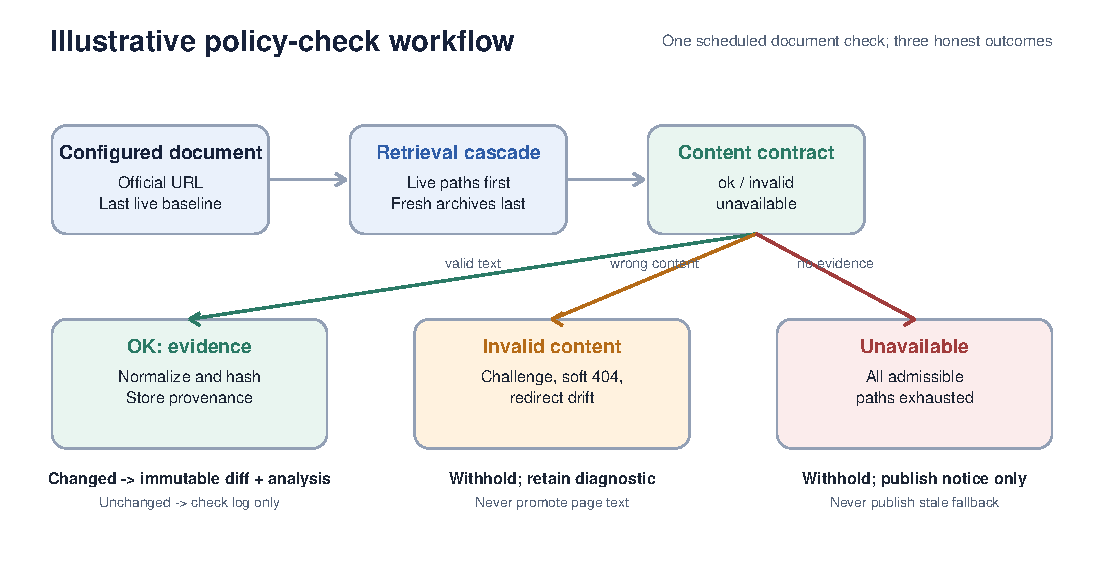
\includegraphics[width=\textwidth]{figures/illustrative-workflow.pdf}
\caption{One document check produces evidence, a diagnosed invalid response, or
explicit unavailability. Only the evidence branch can reach publication.}
\label{fig:workflow}
\end{figure}

A fixture-only installation provides a second example. Its configured records
have realistic shapes for interface development but are marked as seeded and
lack retrieved evidence. Querying the same public APIs used in production yields
zero public policies, zero changes, and suspension notices for every configured
record. This control exercises the boundary independently of provider network
conditions.

\section{Impact}
\label{sec:impact}

The principal impact is methodological: \pw{} makes acquisition uncertainty a
queryable part of the dataset instead of an exception hidden in scanner logs.
Researchers can separate configured coverage from evidence coverage, compare
retrieval-path dependence across providers, examine the duration and causes of
source unavailability, and construct longitudinal corpora whose records retain
source, capture time, normalization path, and publication decision. The same
design supports experiments on change-detection accuracy and human agreement
without conflating a failed fetch with a negative observation.

Table~\ref{tab:impact} reports a dated, reproducible operational snapshot. On
11 July 2026, the running deployment contained 50 configured documents from 16
providers. Forty-six records passed the public-evidence gate and four were
suspended. The public inventory contained 21 change records. Among the 46 public
records, 40 used direct retrieval, five used the renderer, and one used an
archive path. The fixture control exposed no policy or change content. The JSON
snapshot and its read-only collection script are supplied with the submission.

\begin{table}[!ht]
\centering
\small
\begin{tabularx}{\textwidth}{@{}Yrr@{}}
\toprule
\textbf{Operational measure} & \textbf{Production} & \textbf{Fixture control} \\
\midrule
Configured policy records & 50 & 50 \\
Records admitted as public evidence & 46 (92\%) & 0 (0\%) \\
Suspended records & 4 (8\%) & 50 (100\%) \\
Publicly listed providers & 15 of 16 & 0 of 16 \\
Public change-record inventory & 21 & 0 \\
\bottomrule
\end{tabularx}
\caption{Public operational state captured on 11 July 2026. Inventory counts
are not estimates of semantic or legal accuracy.}
\label{tab:impact}
\end{table}

The operational deployment shows that the fallback paths are exercised rather
than merely specified. It also demonstrates that withholding is observable:
unavailable documents remain counted and diagnosable instead of disappearing
from the denominator. The software runs on shared application hosting plus a
small renderer service, so longitudinal collection is feasible without a large
institutional cluster.

For research practice, \pw{} can contribute in four ways. First, it can produce
timestamped provider-version corpora for policy and digital-governance studies.
Second, its per-attempt logs support controlled ablations of direct, HTTP/2,
rendered, and archive retrieval. Third, its explicit negative states allow
measurement of source accessibility and censorship-by-friction without treating
blocked pages as missing at random. Fourth, its normalized diffs and evidence
links can support blinded human annotation of substantive changes and evaluation
of downstream summaries.

The current evidence does not establish precision or recall for semantic change
detection, agreement with legal experts, or correctness of generated risk
annotations. There is not yet a validated claim of broad external adoption, and
the 21 public change records are inventory items rather than independently
adjudicated legal events. These boundaries define the next evaluations: a
pre-registered repeated-scan window, a versioned ground-truth corpus, cascade
ablation, at least two independent annotators, and reporting of agreement,
precision, recall, false-change rate, and time to detection.

The project is publicly developed on GitHub \cite{policywatcher}, provides
installation and contribution documentation, and holds a passing OpenSSF Best
Practices self-assessment \cite{openssf}. These are engineering-quality and
reusability signals, not security or legal certifications. The software is
designed for extension through new providers, policy types, jurisdictions,
retrieval strategies, public views, and analysis backends.

\section{Conclusions}
\label{sec:conclusions}

\pw{} provides an open implementation of evidence-aware monitoring for online
terms and privacy policies. Its reusable contribution is the combination of a
multi-path acquisition cascade, deterministic content contract, freshness rule,
provenance-preserving version store, and shared public-evidence gate. Together,
these mechanisms keep retrieval failures and development fixtures from becoming
apparently authoritative public records. The software is already deployed and
supplies reproducible operational evidence, while its explicit limitations leave
legal and semantic validity to properly designed expert and longitudinal studies.

\section*{Data availability}

The operational snapshot supporting Table~\ref{tab:impact}, together with the
read-only collection script and interpretation notes, is supplied as
Supplementary Data and in the submission source archive. The live public
endpoints are available at \url{https://www.policywatcher.online}. No private
check logs, subscriber information, credentials, administrative data, or raw
provider text are included.

\section*{CRediT author statement}

Fabrizio Degni: Conceptualization, Methodology, Software, Validation,
Investigation, Data curation, Visualization, Writing - original draft, Writing -
review and editing, Project administration.

\section*{Funding}

This research received no specific grant from funding agencies in the public,
commercial, or not-for-profit sectors.

\section*{Declaration of competing interest}

Fabrizio Degni is the creator and maintainer of PolicyWatcher and operates the
public demonstration service. The author declares no financial interest that
could have appeared to influence the work reported in this paper.

\section*{Declaration of generative AI and AI-assisted technologies in the manuscript preparation process}

During the preparation of this work, the author used OpenAI Codex to assist with
editorial restructuring, language refinement, LaTeX preparation, and generation
of reproducible vector-figure source. The author reviewed, verified, and edited
the resulting material and takes full responsibility for the content of the
publication.

\section*{Acknowledgements}

The author thanks the open-source maintainers and public-interest archival
services on which the software depends.

\begin{thebibliography}{00}

\bibitem{mcdonald2008}
A. M. McDonald, L. F. Cranor, The cost of reading privacy policies,
I/S: A Journal of Law and Policy for the Information Society 4 (3) (2008) 543-568.

\bibitem{obar2020}
J. A. Obar, A. Oeldorf-Hirsch, The biggest lie on the internet: ignoring the
privacy policies and terms of service policies of social networking services,
Information, Communication \& Society 23 (1) (2020) 128-147.
\href{https://doi.org/10.1080/1369118X.2018.1486870}{doi:10.1080/1369118X.2018.1486870}.

\bibitem{wilson2016}
S. Wilson, F. Schaub, A. A. Dara, F. Liu, S. Cherivirala, P. G. Leon, et al.,
The creation and analysis of a website privacy policy corpus, in: Proceedings
of the 54th Annual Meeting of the Association for Computational Linguistics,
2016, pp. 1330-1340.
\href{https://doi.org/10.18653/v1/P16-1126}{doi:10.18653/v1/P16-1126}.

\bibitem{amos2021}
R. Amos, G. Acar, E. Lucherini, M. Kshirsagar, A. Narayanan, J. Mayer, Privacy
policies over time: curation and analysis of a million-document dataset, in:
Proceedings of The Web Conference, 2021, pp. 2165-2176.
\href{https://doi.org/10.1145/3442381.3450048}{doi:10.1145/3442381.3450048}.

\bibitem{harkous2018}
H. Harkous, K. Fawaz, R. Lebret, F. Schaub, K. G. Shin, K. Aberer, Polisis:
automated analysis and presentation of privacy policies using deep learning,
in: Proceedings of the 27th USENIX Security Symposium, 2018, pp. 531-548.

\bibitem{lippi2019}
M. Lippi, P. Pa\l{}ka, G. Contissa, F. Lagioia, H.-W. Micklitz, G. Sartor,
P. Torroni, CLAUDETTE: an automated detector of potentially unfair clauses in
online terms of service, Artificial Intelligence and Law 27 (2) (2019) 117-139.
\href{https://doi.org/10.1007/s10506-019-09243-2}{doi:10.1007/s10506-019-09243-2}.

\bibitem{tosdr}
Terms of Service; Didn't Read, ToS;DR public service and data,
\url{https://tosdr.org}, accessed 23 July 2026.

\bibitem{tosback}
Electronic Frontier Foundation, TOSBack: the terms-of-service tracker,
\url{https://tosback.org}, accessed 23 July 2026.

\bibitem{wayback}
Internet Archive, Wayback Machine, \url{https://web.archive.org}, accessed 23
July 2026.

\bibitem{commoncrawl}
Common Crawl Foundation, Common Crawl corpus,
\url{https://commoncrawl.org}, accessed 23 July 2026.

\bibitem{owasp}
Open Worldwide Application Security Project, Server Side Request Forgery
Prevention Cheat Sheet, \url{https://cheatsheetseries.owasp.org/cheatsheets/Server_Side_Request_Forgery_Prevention_Cheat_Sheet.html},
accessed 23 July 2026.

\bibitem{policywatcher}
F. Degni, PolicyWatcher version 3.6.4 [computer software], GitHub, 2026,
\href{https://github.com/sev7enITA/policywatcher/tree/1171b06a119954343c9a9124df4bdfdc9aab4a6d}{GitHub commit 1171b06}.

\bibitem{openssf}
OpenSSF Best Practices Badge Program, PolicyWatcher project 13465,
\url{https://www.bestpractices.dev/projects/13465}, accessed 23 July 2026.

\end{thebibliography}

\section*{Current executable software version}

The public deployment is available at \url{https://www.policywatcher.online}.
Installation and execution instructions for the reproducible source release are
provided in the repository linked in Table~\ref{tab:metadata}.

\end{document}
